\section{Implementação} \label{sec:implementação}

    Durante esta secção irá ser descrito o algoritmo de sincronização e, posteriormente, a sua implementação em Python. Para além disso, é feita a seguinte distinção entre três relógios:
    
    \begin{itemize}
        \item \textbf{Relógio monotónico}:  Relógio do hardware do computador. Nunca é corrigido e conta o tempo a partir do qual o sistema operativo foi iniciado.
        \item \textbf{Relógio NTP}: Relógio do servidor NTP e assumido como correto. Este relógio escraviza o sistema.
        \item \textbf{Relógio abstrato}: Relógio implementado em software em cima do sistema operativo. É o relógio monotónico corrigido em "rate" e "offset" de acordo com a secção \ref{sec:NTP}.
    \end{itemize}

    Posto isto, as raspberrypis têm dois relógios: monotónico e abstrato, sendo que este último é utilizado para tomar as decisões de mudança de estado. O monitor apenas utiliza o seu relógio monotónico para marcar os "timestamps" das mudanças de estado de A e B. O servidor NTP responde aos pedido com os "timestamps" do relógio NTP. A figura \ref{fig:tempo_corrigido} ilustra um pedido de tempo ao relógio relógio abstrato. De referir que, o relógio abstrato é o relógio corrigido segundo os parâmetros obtido pelo último pedido NTP (offset, rate e delay), segundo as equações \ref{eq:parametros} e \ref{eq:corrected_time}.

    \begin{figure}[h]
        \centering
        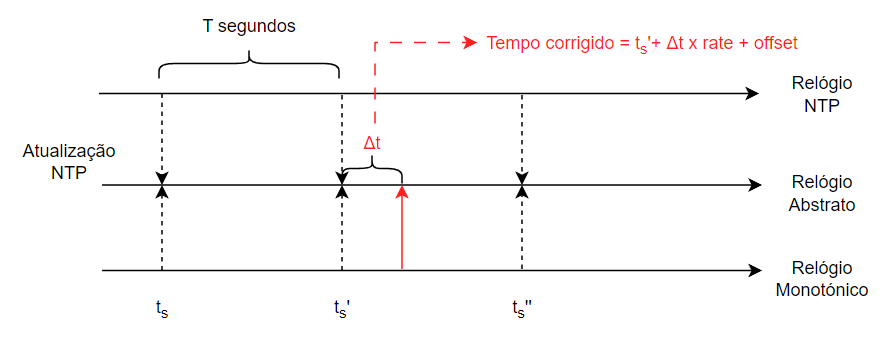
\includegraphics[width=1.0\linewidth]{figures/tempo_corrigido.png}
        \caption{Correção do tempo do relógio abstrato}
        \label{fig:tempo_corrigido}
    \end{figure}

\subsection{Algoritmo}
    O programa está dividido em dois processos distintos que correm em paralelo: correção dos parâmetros do relógio e atualização do Estado. Ambos os algoritmos estão expressos em pseudo-código nas figuras \ref{fig:pseudoCodigoRelogio} e \ref{fig:pseudoCodigoEstado}, respetivamente.
    
    \begin{figure}[h]
        \centering
        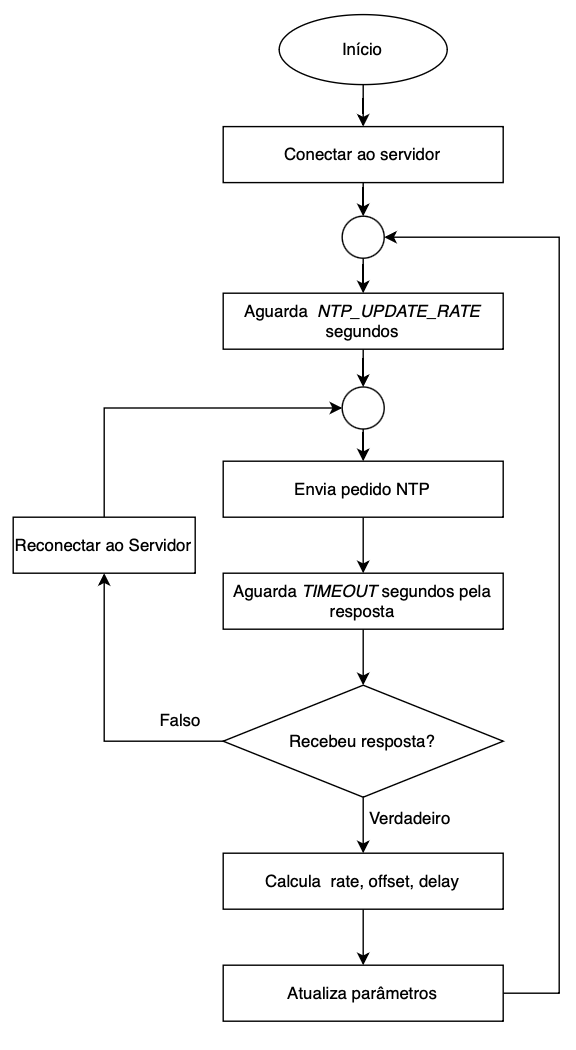
\includegraphics[width=0.55\linewidth]{figures/pseudoCodigoRelogio.png}
        \caption{Pseudo-código relativo à correção do relógio abstrato}
        \label{fig:pseudoCodigoRelogio}
    \end{figure}

    \begin{figure}[h]
        \centering
        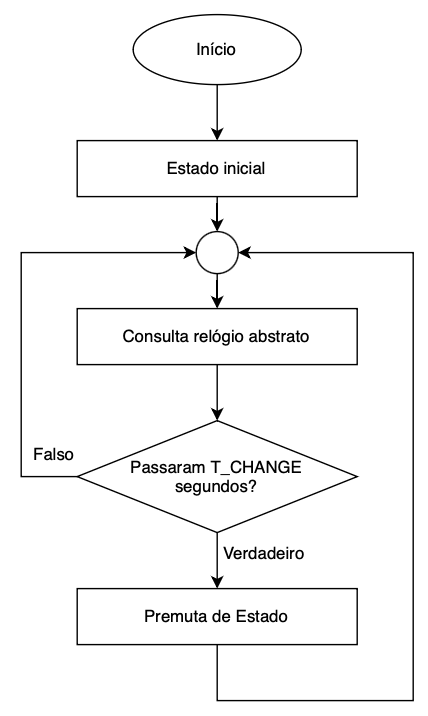
\includegraphics[width=0.55\linewidth]{figures/pseudoCodigoEstado.png}
        \caption{Pseudo-código relativo à atualização do estado}
        \label{fig:pseudoCodigoEstado}
    \end{figure}


\subsection{Implementação em Python}

    O algoritmo foi implementado na linguagem Python. A sincronização NTP foi feita por uma thread periódica, sendo que a sua periodicidade é definida pelo utilizador na invocação do programa. Adicionalmente, 
    o utilizador também pode definir o sentido a que o semáforo
    corresponde e o servidor NTP a que se pretende conectar. O programa consiste em 3 classes que descrevem o relógio abstrato, o cliente NTP e o monitor.
    